%% LyX 2.2.3 created this file.  For more info, see http://www.lyx.org/.
%% Do not edit unless you really know what you are doing.
\documentclass[english]{article}
\usepackage{newcent}
\renewcommand{\familydefault}{\rmdefault}
\usepackage[T1]{fontenc}
\usepackage[latin9]{inputenc}
\usepackage[a4paper]{geometry}
\geometry{verbose,tmargin=2.5cm,bmargin=2.5cm,lmargin=2.5cm,rmargin=2.5cm}
\usepackage{xcolor}
\definecolor{note_fontcolor}{rgb}{0.800781, 0.800781, 0.800781}
\usepackage{babel}
\usepackage{calc}
\usepackage{url}
\usepackage{graphicx}
\usepackage[unicode=true,pdfusetitle,
 bookmarks=true,bookmarksnumbered=false,bookmarksopen=true,bookmarksopenlevel=1,
 breaklinks=false,pdfborder={0 0 0},pdfborderstyle={},backref=false,colorlinks=false]
 {hyperref}
\hypersetup{
 urlcolor=marineblue  linkcolor=blue}

\makeatletter

%%%%%%%%%%%%%%%%%%%%%%%%%%%%%% LyX specific LaTeX commands.
%% Because html converters don't know tabularnewline
\providecommand{\tabularnewline}{\\}
%% The greyedout annotation environment
\newenvironment{lyxgreyedout}
  {\textcolor{note_fontcolor}\bgroup\ignorespaces}
  {\ignorespacesafterend\egroup}

%%%%%%%%%%%%%%%%%%%%%%%%%%%%%% Textclass specific LaTeX commands.
\newenvironment{lyxlist}[1]
{\begin{list}{}
{\settowidth{\labelwidth}{#1}
 \setlength{\leftmargin}{\labelwidth}
 \addtolength{\leftmargin}{\labelsep}
 \renewcommand{\makelabel}[1]{##1\hfil}}}
{\end{list}}

%%%%%%%%%%%%%%%%%%%%%%%%%%%%%% User specified LaTeX commands.
\usepackage{url}

%used by keystroke
\usepackage{array}
\usepackage{keystroke}
%\usepackage[os=win]{menukeys}

\makeatother

\usepackage{listings}
\renewcommand{\lstlistingname}{Listing}

\begin{document}

\title{InetVis 2.1.1 Manual}
\maketitle
\begin{center}

\includegraphics{images/icon}
\par\end{center}

\tableofcontents{}

\section{Description}
\begin{description}
\item [{InetVis}] -\textbf{ I}nter\textbf{net} \textbf{Vis}ualization
\item [{Version}] 2.1.1 
\item [{Rrelease~Date:}] 2017/10/09
\end{description}
InetVis is a 3-D scatter-plot visualization for network traffic. Inetvis
is more or less like a media player, but for network traffic. At the
moment its just an academic toy for reviewing packet capture files,
but may be useful in other endeavours. For example, InetVis has been
used to verify and critique the accuracy of scan detection algorithms
in the Snort IDS and Bro IDS.

\subsection{About}

Inetvis was originally developed in 2005-2007, as part of a research
project by JP van Riel in the Department of Comuter Science at Rhodes
Uinversity. 10 years later the project has been resurected by Yestin
Johnson as part of his Masters Degree research. both Projects have
been supervised by Barry Irwin. 

The Current version of Inetvis (2.x branch) has been ported across
to run on Qt5.x (including Qt5.5) and on modern operating systems,
and is now hosted on GitHub.

Current Author: Yestin Johnson (2017) <yestinj@gmail.com>

Reseach Supervisor: Barry Irwin

Institute: Department of Computer Science,

Rhodes University,

Github: \url{https://github.com/yestinj/inetvis}

Original Inetvis Concept Paper: \url{https://doi.org/10.1145/1108590.1108604}

\subsubsection{Inetvis 0.9.x and 1.x (unreleased)}

Original Author (InetVis 1.x): Jean-Pierre van Riel (2005 - 2007)
<jp.vanriel@gmail.com>

Website: http://research.ict.ru.ac.za/G02V2468/

Grahamstown, 6140, Eastern Cape, South Africa

\subsection{Concept}

The original source of inspiration for InetVis is the \textquotedbl{}\emph{The
Spinning Cube of Potential Doom}\textquotedbl{} (by Stephen Lau).
Whilst many other network visualizations employ lines as a metaphor
for connection, the 3-D scatter-plot of points proves to scale well
with larger volumes of data. The visualization makes network scanning
and port scanning readily evident as horizontal and vertical lines
respectively. InetVis offers numerous extensions that enhance the
original basic concept. 

Lau's Original Paper: \url{ https://doi.org/10.1145/990680.990699}

Original Article:\url{ http://www.nersc.gov/news-publications/nersc-news/nersc-center-news/1998/cube-of-doom/}

\subsection{ Input}

InetVis visualizes packet captures of network traffic using Libpcap
to either
\begin{itemize}
\item capture live traffic from the default interface
\item replay traffic from a pcap file.
\end{itemize}
Tcpdump (\url{http://www.tcpdump.org}), Wireshark (\url{http://wireshark.org})
and Snort (\url{http://www.snort.org}) are examples of other applications
can use and produce network packet captures in the Libpcap file format.

\subsection{Supported Protocols}

Currently only Ethernet based IPv4 packets are supported. Within the
TCP/IP suite explicit support is provided for TCP, UDP and ICMP protocols.
Other protocols may be silently dropped by the builtin base BPF filter
(\textquotedbl{}\texttt{\textsl{ip{[}6:2{]} \& 0x3fff\textquotedbl{}}}).
See Section 4.2 for details.

\subsection{Plotting scheme}
\begin{enumerate}
\item Destination address (home network) plotted along blue x-axis (horizontal).
\item Source address (external Internet range) plotted along red z-axis
(depth). 
\item Ports (TCP and UDP) plotted along green y-axis (vertical). 
\item ICMP traffic plotted below TCP/UDP cube grey/white ICMP plane.
\end{enumerate}
\begin{center}
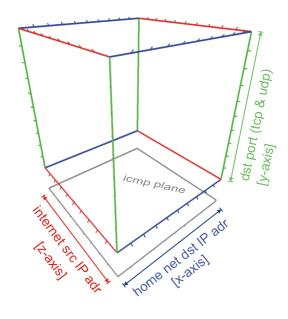
\includegraphics[scale=0.3]{images/inetvis_plotting_scheme}
\par\end{center}

\subsection{Features}
\begin{itemize}
\item Adjustable replay position to seek through the traffic capture files.
\item Variable playback speed (time scaling), from as slow as 0.001x (1
ms/s), or as fast as 86400x (1 day/s).
\item Variable time frame/window to view events for the past 100 ms up to
5 years.
\item Transparent decay of events - points fade as they age (with respect
to the time window).
\item New events are highlighted by pulsing once (a momentarily bulge of
the point). 
\item Filtering capability via BPF filter expressions (as used in Libpcap
and Tcpdump).
\item Various colour schemes for colouring points and adjustable point size.
\item Setting the data ranges and scaling down into sub-domain IP addresses
(destination and source) as well as port ranges to view a subset of
the traffic data.
\item Adjustable logarithmic plot for stretching out (thus increasing visibility)
lower port range where, in general, most TCP/UDP traffic occurs.
\item Various reference frame controls, i.e. toggling visibility of axes,
markers, transparent grid lines, labels, and background colour. 
\item Orthographic and perspective projection modes. 
\item Immersive navigation - scaling (zooming), translating (moving) and
rotating. 
\item Record single snapshot image, or dump all image frames (useful for
manually encoding video clips). 
\item Record output back to pcap binary file format, for further detailed
analysis with other applications (e.g. Tcpdump, Wiresahark and Snort).
\end{itemize}
See the CHANGELOG file in the source distribution for updated feature
additions.

\section{Usage}

\subsection{Command Line}

\texttt{\$ ./inetvis }

Inetvis takes no commandline arguments at this time.

\subsection{User Interface and Controls}

The display pane and control panel are in separate windows, with a
plotter settings dialogue and reference frame settings dialogue accessed
via the 'view' menu of the control panel

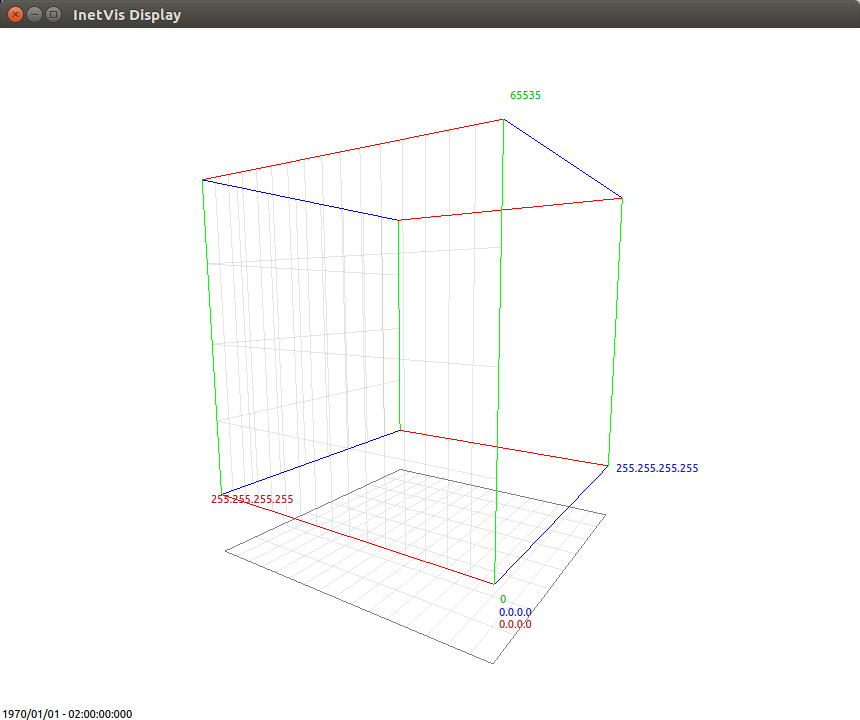
\includegraphics[scale=0.3]{images/InetvisDisplay}

\subsubsection{Control Panel}

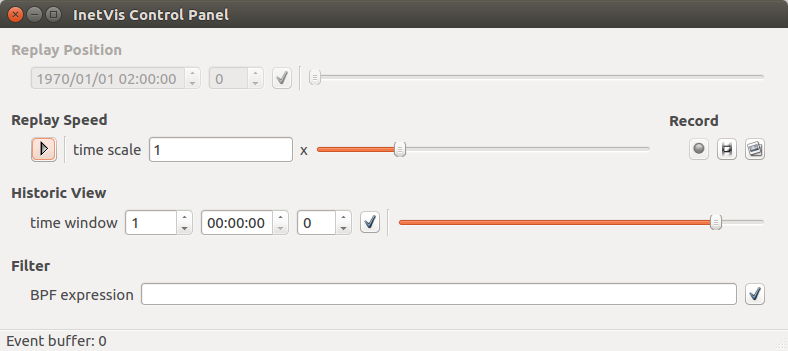
\includegraphics[scale=0.5]{images/InetVisControlPanel}
\begin{itemize}
\item main menu to open files, set mode (monitor local host or replay file),
or to access other dialogues (view).
\item Replay position controls. 
\item Playback and replay speed controls. 
\item Recording controls. 
\item Time window controls (Historic View). 
\item Filter.
\item Task-bar reports the number of packets currently in the buffer.
\end{itemize}

\subsection{InetVis Display}

This is the primary visualization display pane.

\subsubsection{Navigation via Mouse Controls}
\begin{itemize}
\item Holding left button and moving rotates. 
\item Holding right button and moving translates along x and y (horizontally
and vertically respectively). 
\item Rotating scroll wheel translates along z (depth). 
\item Holding middle button and moving zooms.
\end{itemize}

\subsubsection{Navigation via Keyboard Controls}
\begin{itemize}
\item   \LArrow\UArrow\DArrow\RArrow to rotate the cube.
\item  \Ctrl +   \LArrow\UArrow\DArrow\RArrow  to translate (x and y). 
\item  \Alt+\UArrow or  \Alt+\DArrow to translate (z). 
\item \keystroke{+} and \keystroke{-}to scale (zoom). 
\item  \Ctrl + \keystroke{L} Set Left View (up \emph{x} axis)
\item  \Ctrl + \keystroke{R} Set Right View (down \emph{x} axis) 
\item  \Ctrl + \keystroke{T} Set Top View (down\emph{ y} axis) 
\item  \Ctrl + \keystroke{B} Set Bottom View (up\emph{ y} axis)
\item  \Ctrl + \keystroke{F} Set Front View (up\emph{ x} axis) 
\item  \Home Set Front view (down\emph{ y} axis)
\item  \End Set Back View (down\emph{ z} axis)
\end{itemize}

\subsubsection{Other Keyboard Controls}
\begin{itemize}
\item  \keystroke{F} Toggle full screen. 
\item  \Esc Exit full screen 
\item  \keystroke{$\sim$}  Toggle \emph{Harlemshake} 
\item  \keystroke{0} Clear the visualisation pane 
\item  \keystroke{1} Rotation Toggle 
\item  \keystroke{2} Decrease Rotation 
\item  \keystroke{3} Increase Rotation 
\item \keystroke{9} Toggle FPS display
\item  \Ctrl + \keystroke{H} Hide Home Range (addresses prefix replaced
with \emph{the.drk.net}) 
\item  \keystroke{F} Take single frame Screenshot 
\item  \Spacebar Pause/Resume the visualisation 
\item  \Ctrl + \keystroke{Q} Quit the application 
\item \keystroke{P} to bring up Plotter Settings Dialogue. 
\item  \keystroke{R} to bring up Reference Frame Settings Dialogue. 
\item  \keystroke{C} to bring up Control Panel Dialogue. 
\end{itemize}

\subsection{ Plotter Settings Dialogue}
\begin{center}
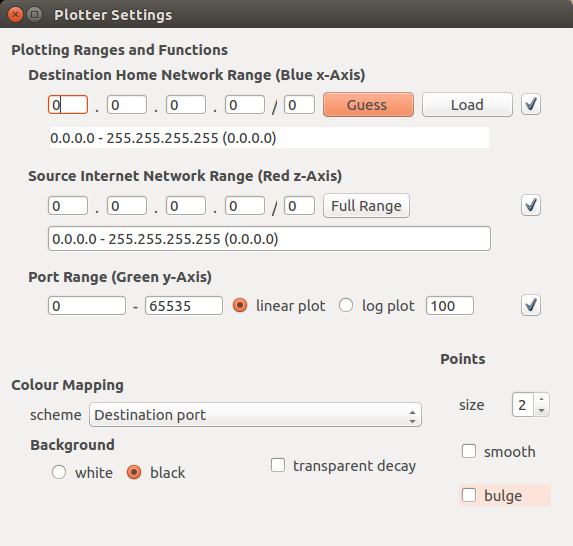
\includegraphics[scale=0.5]{images/PlotterSettings}
\par\end{center}
\begin{itemize}
\item Set the destination home network range (or drill down into it).
\item Set the source Internet range (drill down into a domain).
\item Set the port range (drill down into a port range). 
\item Set linear or logarithmic plotting for ports. 
\item Set colour mapping, toggle transparent decay, and set background colour
(black or white). 
\item Set point size, point bulging (highlight new events), and toggle point
smoothing (rounded points).
\end{itemize}

\subsection{Reference Frame Settings Dialogue}
\begin{center}
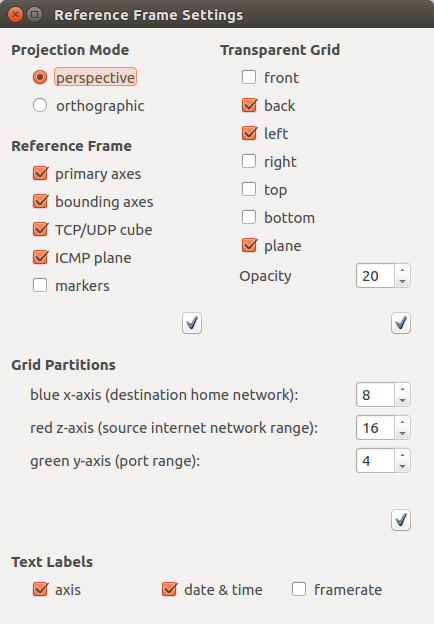
\includegraphics[scale=0.5]{images/ReferenceFrameSettings}
\par\end{center}
\begin{itemize}
\item Set projection mode (Orthographic or perspective). 
\item Toggle visibility of reference frame axes and markers. 
\item Toggle visibility and transparency of grid lines. 
\item Set number of divisions along \emph{x}, \emph{y}, and\emph{ z} for
markers and grid lines. 
\item Toggle text labels (time, axes ranges, frame rate).
\end{itemize}

\subsection{General Settings Dialogue}

New functionalituy addedin in version 2.1.0 is the ability to have
inetvis save a config file. The location of this file depends on the
way QT handles it in a patfrom specific manner
\begin{lyxlist}{00.00.0000}
\item [{Ubuntu}] \textasciitilde{}/.config/Rhodes\textbackslash{} University/InetVis.conf
\item [{MacOSX}] <todo>
\item [{Windows}] <todo>
\end{lyxlist}
An example of a default config file is shown below.

\begin{lstlisting}[basicstyle={\footnotesize\ttfamily},breaklines=true,showspaces=true]
[dataproc]
home_network\default_home_network=0.0.0.0/0
home_network\monitor_interface=
home_network\show_not_set_error=false
recording\default_dir=inetvis-recorded
recording\frames_subdir=inetvis-recorded/frames
recording\live_subdir=live
recording\pcaps_subdir=inetvis-recorded/pcaps
recording\replay_subdir=replayed 
recording\snapshots_subdir=inetvis-recorded/snapshots 
screenshot\screenshot_extension=png
screenshot\screenshot_format=png
screenshot\screenshot_quality=-1

[glviswidget]
pos=@Point(186 127)
size=@Size(704 605)

[logging]
root_dir=logs
stderr_filename=stderr
stdout_filename=stdout 
\end{lstlisting}


\subsubsection{Record Settings}
\begin{center}
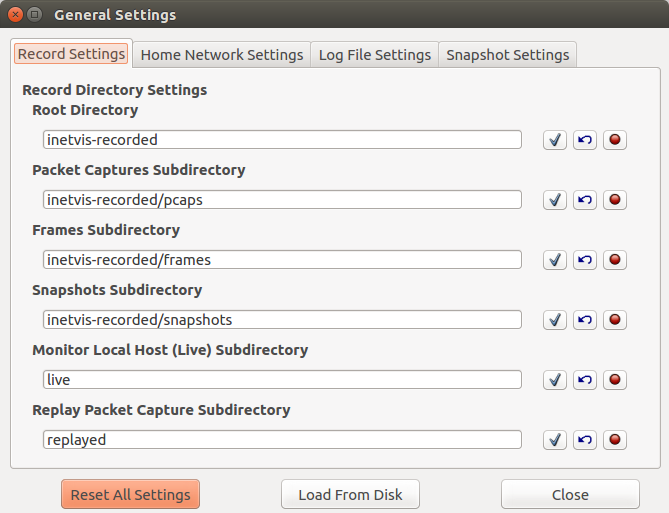
\includegraphics[scale=0.5]{images/RecordSettings}
\par\end{center}

These directories are all relative to the directory in which inetvis
is run.

\subsubsection{Home Network settings}
\begin{center}
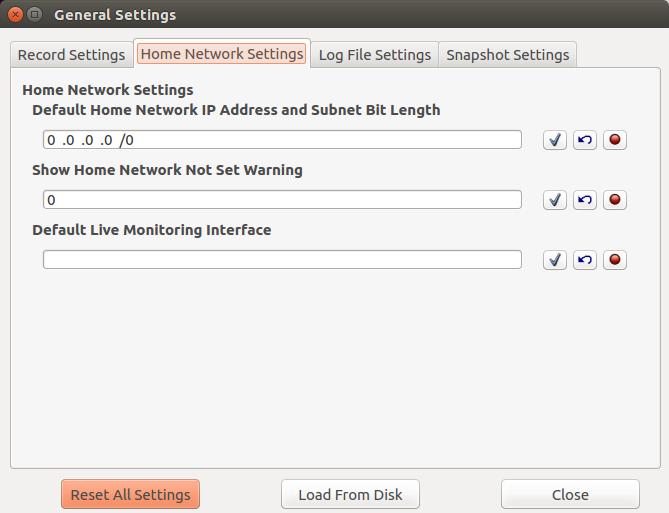
\includegraphics[scale=0.5]{images/HomeNetworkSettings}
\par\end{center}

Dialogs for setting the home network ( useful if the same network
is being monitored )

\subsubsection{Log File Settings}
\begin{center}
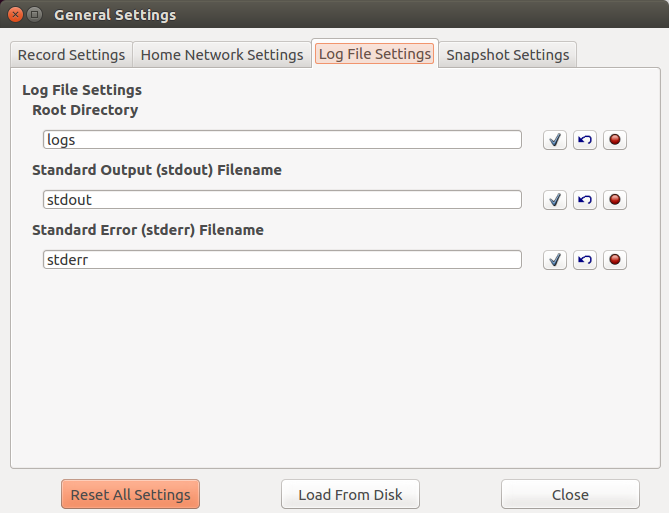
\includegraphics[scale=0.5]{images/LogFileSettings}
\par\end{center}

Logging data relative to startup directory

\subsubsection{Snapshot Settings}
\begin{center}
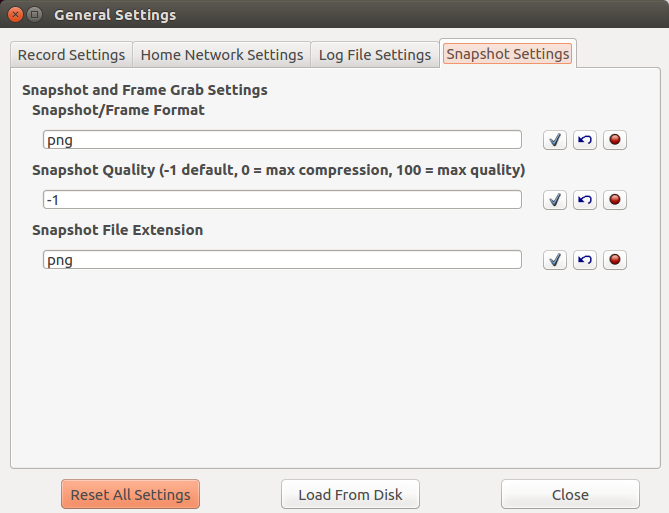
\includegraphics[scale=0.5]{images/ScreenShotSettings}
\par\end{center}

Format and configuration to support screenshots. PNG, BMP, and PPM
formats are now supported.

\section{Usage Notes}

\subsection{Tool tips as Helpful Hints}

Majority of the controls, buttons and fields in the GUI provide tool
tips to help explain their function and usage. Tool tips can be seen
by hovering the mouse cursor over the GUI component in question.

\subsection{Applying Settings}

Many of the settings are grouped together and require the user to
click the apply button (button with a tick icon) once they are ready
to apply the new settings.

\subsubsection{Setting the Home Network Range Before Playback}

After opening a file, set the home network address (in Plotter Settings
dialogue) to scale the data along the blue axis - otherwise all traffic
is rendered in a narrow single band with respect to the x-axis. A
'guess' button can help infer this home network range by checking
the destination addresses contained within the file. In the case of
monitoring the local network interface (live packet capture), the
application will automatically retrieve the home network address from
Libpcap.

\subsubsection{Setting Address Ranges with CIDR Notation}

Setting the address ranges entails using 'dots-slash' (CIDR) notation
to specify network sub-domains. For example 192.168.0.0/24 is the
network with address 192.168.0.0, subnet mask 255.255.255.0, giving
the network range 192.168.0.0 to 192.168.0.255\textbackslash{}. The
number after the slash represents the number of bits in the subnet
mask. Thus the octet classed network masks are:
\begin{lyxlist}{00.00.0000}
\item [{Legacy~Class~A}] 255.0.0.0 = /8 
\item [{Legacy~Class~B}] 255.255.0.0 = /16 
\item [{Legacy~Class~C}] 255.255.255.0 = /24
\end{lyxlist}
Values other than /8, /16 and /24 are trickier as they involve bits
in between the four octets of a 32 bit IP address. The Plotter Settings
dialogue has a field below the dots-slash edit boxes that show the
range and subnet mask to help as guide. For bits added on to a full
octet (i.e. /8+x or /16+x or /24+x), the following octet in the mask
will have the value:

\begin{tabular}{|c|c|c|c|c|c|c|}
\hline 
/+1 & /+2 & /+3 & /+4 & /+5 & /+6 & /+7\tabularnewline
\hline 
\hline 
.128 &  .192 &  .224 & .240 &  .248 & .252 & .254\tabularnewline
\hline 
\end{tabular}

For example, 192.168.120/20 has subnet mask 255.255.248.0 and represents
8 /24 (Legacy Class C) networks in the range 192.168.120.0 to 192.168.127.255.

\subsection{Recording}

All three record methods, recording to capture file, taking a single
image snapshot, or dumping rendered frames to image files, can be
used simultaneously and used in conjunction with playback.

Recording back to capture file, taking a snapshot image, or dumping
frames, creates a directory hierarchy relative to the InetVis running
directory.
\begin{lyxlist}{00.00.0000}
\item [{recorded/frames}] Sequences of framed which can be stiched together
to create video
\item [{recorded/pcaps}] files in pcap format
\item [{recorded/snapshots}] individual image snapshots
\end{lyxlist}
Within these directories, sub-directory structures follow and should
be self explanatory. Some file and directory names include numeric
timestamps of the form yyyymmdd-hhMMsszzz (where MM is minutes and
zzz milliseconds) - the timestamps refer to timestamps in the capture
file (or live capture).

\subsubsection{Record to Capture File}

InetVis can record back out to a Libpcap packet capture file which
can later be reviewed with any other tool capable of reading the file
format (e.g. Wireshark or tcpdump). A record session begins when the
record button (with the round red record symbol) is toggled on, and
stops once the button its toggled off. Everything seen in the current
display (and time window), as well as any consequent playback, will
be recorded while the red record button is toggled on.

\subsubsection{Taking an Image Snapshot}

Pressing the record button with a picture symbol allows the user to
take a snapshot of the current image in the visualization pane of
the InetVis Display window. To save a single frame to disk the \keystroke{Z}
key can be used when uin the plotter window.

\subsubsection{Dumping Rendered Frames to Image Files}

InetVis can record rendered frames to image files. Frame record sessions
work much the same way as capture file record sessions. Whilst the
record button with the film symbol is on, the application dumps each
frame to an image file, and stops when the button is toggled off.
For each frame, a raw copy of the image buffer is copied into an uncompressed
image file (.ppm format). Consequently, recording image frames uses
up a large amount of disk space at a rapid rate and can degrade the
applications performance - setting the window to a smaller resolution
will help reduce the performance hit. During frame recording, the
timing is fixed to produce frames suitable for encoding video clips
at 25 frames per second (fps). Even if, whilst recording, it appears
that playback is degraded to less than 25 fps, the timing between
each frames is calculated with respect to the data in the file and
according to the replay speed. Therefore, when the frame capture files
are encoded to video a clip at 25 frames per second, the video clip
has the correct timing and replay speed while despite the recording
process appearing slower. As a consequence, playback of some video
clips may appear faster that the original recording.

\subsection{Minimum System Specification}

The Original system was devloped with very modidst hardware requirements
by modern standards (see below). Performance on more modern multicore
systems is very good, and able to achieve frame rates of 25 FPS even
using software rendering in a virutal machine. Siginificant performance
hits still occur when dumping successive fames to disk (this is especially
evident when using the PNG file format).\\

\noindent\fcolorbox{black}{lightgray}{\begin{minipage}[t]{1\columnwidth - 2\fboxsep - 2\fboxrule}%
\textbf{InetVis 0.9.x Requirements:}

At least a Pentium III class processor with 256MB RAM and a 3-D graphics
accelerator supporting OpenGL is recommended. 

While InetVis may work with on-board video cards, poor performance
and limited OpenGL support is a typical drawback.

Typical Performance:
\begin{itemize}
\item Tested on Ubuntu 7.04 with Intel Core2 (6300) 1.86 GHz CPU, 2GB RAM,
GeForce 7600GS (256MB) graphics card.
\item The application takes a best effort approach to rendering 25 frames
a second. Once rendering at less than 25 frames per second, playback
becomes slower than the chosen replay rate. 
\item During playback, handles 100MB capture file with about 500,000 packets
at 25 frames per second. 
\item During playback, handles 200MB capture file with about 2,000,000 packets
at about 5 FPS. 
\item When paused, handles 600MB capture file with about 6,000,000 packets
at 8 FPS using an OpenGL display list optimisation. 
\item When recording frames, expect a significant performance hit due to
heavy file I/O.
\end{itemize}
%
\end{minipage}}

\section{Known Issues}

As of Version 2.1.0 the following known issues are still present:
\begin{itemize}
\item At present running the standalone app does not work on Mac OS, however
opening with Qt Creator, building, and then running does work. 
\item Monitoring local network interfaces does not work under Mac OS at
this time. 
\item Windows support is failing to compile.
\end{itemize}

\subsection{Stability and Performance}
\begin{enumerate}
\item Target frame rate is intentionally caped at 25 frames per second.
The achieved frame rate is usualy a little slower and when the system
reaches full processor usage, the replay rate is reduced to a best
effort (plays slower than the chosen replay rate). 
\item Large capture files can take a while to load while the GUI remains
unresponsive. Similarly, some interactions require reloading the capture
file, which, if not cached in RAM, will be applied with noticeable
delay. This is minimised on modern systems with sufficient RAM
\item Attempting to view too many packets may exhaust system memory. The
system will just about halt if the application starts running from
swap space. (unlikley with >4GB ram)
\begin{enumerate}
\item To improve InetVis should (yet to be implemented) have a memory cap
set and warn the user while automatically decreasing the time window
to limit memory usage.
\end{enumerate}
\item The Microsoft Windows (currently broken) and MacOS port is, not tested
extensively and expected to be buggy. 
\item Live monitoring is still has a few heisenbugs See \url{https://github.com/yestinj/inetvis/issues/46}.
\end{enumerate}
A Full list of current issues can be found on \href{https://github.com/yestinj/inetvis/issues}{GitHub}
\url{https://github.com/yestinj/inetvis/issues}.

\subsection{Limitations and Feature Wish List}
\begin{enumerate}
\item The option to aggregate packet traffic into flows would be a major
improvement for dealing with production class network traffic. 
\item Additional colour schemes would be nice. Furthermore, colour legends
would help assist the users interpreting colours. 
\item Axes labels overlap in certain orientations. 
\item The reference frame and grid lines could be made more intelligent
by dynamically scaling according to the data ranges chosen and only
applying grids on the panes of the cube in the background. 
\item Error reporting needs refinement (multiple reports and obscure references
to code functions might be experienced). 
\item InetVis lacks a mechanism to select a point an call up detailed textual
information, such as the IP addresses, ports, and other such details. 
\item The multi-window GUI is a little awkward and could do with re-factoring
into a single integrated window with semi-transparent control overlays.
This would allow the user to toggle controls and while making changes
see the effect on the visualisation in the background. 
\item Would be nice to have a 'play list' of capture files that can be queued
for replay. 
\item Proper file indexing, instead of re-reading the file from the start
would improve manipulations (such as setting the filter, setting the
domain/port ranges, changing the colour scheme, and so forth). 
\item Currently, the application only caters for traffic captured from an
Ethernet data link. 
\item IP packets with options are processed, but the options are ignored.
Fragmented IP packets are not yet handled and simply drooped by an
implicit BPF filter \textquotedbl{}ip{[}6:2{]} \& 0x3fff\textquotedbl{}.
Refer to RFC 791 for details about the fragment flags and offset field. 
\item The ability to integrate IDS alerts, or at least scan detection alerts
from an IDS, would be awesome.
\end{enumerate}
Additional features in 'todo' status can be found on \href{https://github.com/yestinj/inetvis/issues}{GitHub}
\url{https://github.com/yestinj/inetvis/issues?q=is%3Aissue+is%3Aopen+label%3Aenhancement}..

\section{Running Inetvis}

The instructions below have all been tested on the current version
of Ubuntu, 17.04 64-bit. Installing and Running InetVis

A compiled version of InetVis is available under the releases section
of \url{https://github.com/yestinj/inetvis}.

\subsection{Installation}

In order to install and run the software please do the following:
\begin{enumerate}
\item Download the latest release archive from the releases page. 
\item Extract the archive which will be called something like inetvis-2.1.1.tgz 
\item Change into the extracted directory, something like inetvis-2.1.1
\item Run the install\_inetvis.sh shell script to install the software. 
\item This script will: 
\begin{itemize}
\item install the software to /opt/inetvis-<version>
\item Create a symlink directory /opt/inetvis for convenience
\item Copy across the relevant files to the new directory under /opt. 
\item Place an icon file in /usr/share/icons/hicolor/48x48/apps/
\item Place a desktop file in /usr/share/applications, allowing inetvis
to be found in the menu on Ubuntu systems. 
\item Create a symlink at /usr/local/bin/inetvis pointing to the main binary. 
\item Set the cap\_net\_raw, and cap\_net\_admin=eip capabilities on the
inetvis binary allowing for monitoring packets on local host without
running as root. 
\begin{itemize}
\item \texttt{\$sudo setcap 'CAP\_NET\_RAW+eip CAP\_NET\_ADMIN+eip' }
\item This needs to generally not be /home which on Debian/ubuntu systems
is mounted nosuid 
\end{itemize}
\item If the script completes successfully inetvis should now be in your
path, and also be in the menu system of your distribution.
\end{itemize}
\item You should now be able to run the inetvis binary from the command
line, as it will be in your path, or you can run it from the Ubuntu
menu system, where it will show up as an item. Running from the command
line allows you to view console messages produced while the application
is running. 
\end{enumerate}

\subsection{Uninstalling InetVis}

A convenience script is included in the release archive, namely uninstall\_inetvis.sh,
which can be used to completely remove inetvis from your system at
any time.

\subsection{Disclaimer}

This code may eat your homework \textemdash{} \emph{Caveat emptor}
.

\section{Building and Developing InetVis}

In order to build InetVis onn your own system or VM please consider
the following guidelines:
\begin{enumerate}
\item Update your system: 
\begin{enumerate}
\item \texttt{sudo apt-get update} and\texttt{ sudo apt-get upgrade},
\item finally \texttt{sudo apt-get dist-upgrade }
\item Install the following dependencies: \texttt{sudo apt-get install libpcap-dev
qt5-default}
\end{enumerate}
\item It has been noted that the following dependencies were also required
on \emph{Linux Mint} based systems:
\begin{enumerate}
\item \texttt{sudo apt-get install libqglviewer-dev libqglviewer2}
\end{enumerate}
\item Once the dependencies are installed, clone this repository if you
haven't already.
\begin{enumerate}
\item Clone the github repo into the inetvis directory: git clone git@github.com:yestinj/inetvis.git 
\end{enumerate}
\item Change into the inetvis directory, and then change to src. 
\item Checkout whichever branch you want to build, i.e. master or develop.
git checkout master
\item Finally, build the inetvis binary:
\begin{enumerate}
\item qmake ; make
\item This will result in a new inetvis binary being generated within the
source directory.
\end{enumerate}
\item You may now run inetvis by simply running the generated binary. You
will need to either run using sudo, or set packet capture capabilities
(see instructions above) on the file in the event that you would like
to monitor your local host for packets.
\end{enumerate}

\section{Contact}

Any questions/queries can be directed to Yestin Johnson (2017) <yestinj@gmail.com>,
or via GitHub.
\begin{center}
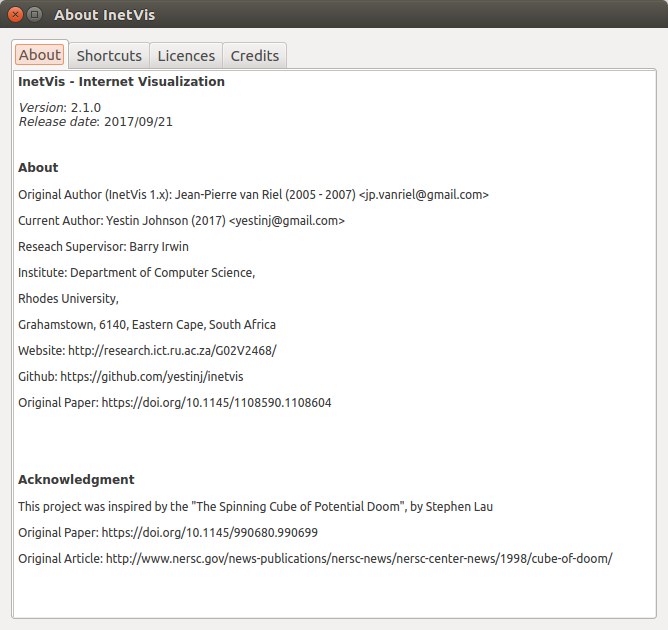
\includegraphics[scale=0.5]{images/About}
\par\end{center}

\section{Credits}

Significant Contributions to this software beyond the base code have
been made by:

Barry Irwin

Alan Herbert

\section{Licence}

\paragraph{\emph{InetVis - Internet Visualisation for network traffic analysis. }}

\paragraph{\emph{Copyright (C) 2005 - 2007, Jean-Pierre van Riel}}

\paragraph{\emph{Copyright (C) 2017, Yestin Johnson, Barry Irwin, Jean-Pierre
van Riel}}

\emph{This program is free software; you can redistribute it and/or
modify it under the terms of the GNU General Public License as published
by the Free Software Foundation; either version 2 of the License,
or (at your option) any later version.}

\emph{This program is distributed in the hope that it will be useful,
but WITHOUT ANY WARRANTY; without even the implied warranty of MERCHANTABILITY
or FITNESS FOR A PARTICULAR PURPOSE. See the GNU General Public License
for more details.}

\emph{You should have received a copy of the GNU General Public License
along with this program; if not, write to the Free Software Foundation,
Inc., 51 Franklin Street, Fifth Floor, Boston, MA 02110-1301, USA.}

\section{Software Dependencies and Licensing}

\begin{lyxgreyedout}
THIS NEEDS TO BE UPDATED%
\end{lyxgreyedout}

InetVis makes use of Libpcap/WinPcap, Qt and OpenGL. The open source
version of Qt by Trolltech is licensed under the GPL, version 2 (as
shown above). According to SGI, use of the OpenGL API requires no
license. Libpcap is distributed under the BSD license. WinPcap, the
windows derivative of libpcap is licensed by CASE Technologies. As
required, the respective licenses are shown below.

\subsection{\textsf{\textsl{\footnotesize{}Libpcap License}}}

\texttt{\textsl{\scriptsize{}License: BSD}}{\scriptsize \par}

\texttt{\textsl{\scriptsize{}Redistribution and use in source and
binary forms, with or without modification, are permitted provided
that the following conditions are met:}}{\scriptsize \par}

\texttt{\textsl{\scriptsize{}1. Redistributions of source code must
retain the above copyright notice, this list of conditions and the
following disclaimer. 2. Redistributions in binary form must reproduce
the above copyright notice, this list of conditions and the following
disclaimer in the documentation and/or other materials provided with
the distribution. 3. The names of the authors may not be used to endorse
or promote products derived from this software without specific prior
written permission.}}{\scriptsize \par}

\texttt{\textsl{\scriptsize{}THIS SOFTWARE IS PROVIDED ``AS IS'' AND
WITHOUT ANY EXPRESS OR IMPLIED WARRANTIES, INCLUDING, WITHOUT LIMITATION,
THE IMPLIED WARRANTIES OF MERCHANTABILITY AND FITNESS FOR A PARTICULAR
PURPOSE.}}{\scriptsize \par}

\subsection*{\texttt{\textsl{\scriptsize{}WinPcap License}}}

\texttt{\textsl{\scriptsize{}Copyright (c) 1999 - 2005 NetGroup, Politecnico
di Torino (Italy). Copyright (c) 2005 - 2007 CACE Technologies, Davis
(California). All rights reserved. Redistribution and use in source
and binary forms, with or without modification, are permitted provided
that the following conditions are met:}}{\scriptsize \par}

\texttt{\textsl{\scriptsize{}1. Redistributions of source code must
retain the above copyright notice, this list of conditions and the
following disclaimer. 2. Redistributions in binary form must reproduce
the above copyright notice, this list of conditions and the following
disclaimer in the documentation and/or other materials provided with
the distribution. 3. Neither the name of the Politecnico di Torino,
CACE Technologies nor the names of its contributors may be used to
endorse or promote products derived from this software without specific
prior written permission.}}{\scriptsize \par}

\texttt{\textsl{\scriptsize{}THIS SOFTWARE IS PROVIDED BY THE COPYRIGHT
HOLDERS AND CONTRIBUTORS \textquotedbl{}AS IS\textquotedbl{} AND ANY
EXPRESS OR IMPLIED WARRANTIES, INCLUDING, BUT NOT LIMITED TO, THE
IMPLIED WARRANTIES OF MERCHANTABILITY AND FITNESS FOR A PARTICULAR
PURPOSE ARE DISCLAIMED. IN NO EVENT SHALL THE COPYRIGHT OWNER OR CONTRIBUTORS
BE LIABLE FOR ANY DIRECT, INDIRECT, INCIDENTAL, SPECIAL, EXEMPLARY,
OR CONSEQUENTIAL DAMAGES (INCLUDING, BUT NOT LIMITED TO, PROCUREMENT
OF SUBSTITUTE GOODS OR SERVICES; LOSS OF USE, DATA, OR PROFITS; OR
BUSINESS INTERRUPTION) HOWEVER CAUSED AND ON ANY THEORY OF LIABILITY,
WHETHER IN CONTRACT, STRICT LIABILITY, OR TORT (INCLUDING NEGLIGENCE
OR OTHERWISE) ARISING IN ANY WAY OUT OF THE USE OF THIS SOFTWARE,
EVEN IF ADVISED OF THE POSSIBILITY OF SUCH DAMAGE.}}{\scriptsize \par}

\texttt{\textsl{\scriptsize{}\_This product includes software developed
by the University of California, Lawrence Berkeley Laboratory and
its contributors. This product includes software developed by the
Kungliga Tekniska Hogskolan and its contributors. This product includes
software developed by Yen Yen Lim and North Dakota State University.\_}}{\scriptsize \par}

\texttt{\textsl{\scriptsize{}{*} {*} {*}}}{\scriptsize \par}

\texttt{\textsl{\scriptsize{}Portions Copyright (c) 1990, 1991, 1992,
1993, 1994, 1995, 1996, 1997 The Regents of the University of California. All
rights reserved.}}{\scriptsize \par}

\texttt{\textsl{\scriptsize{}Redistribution and use in source and
binary forms, with or without modification, are permitted provided
that the following conditions are met:}}{\scriptsize \par}

\texttt{\textsl{\scriptsize{}1. Redistributions of source code must
retain the above copyright notice, this list of conditions and the
following disclaimer. 2. Redistributions in binary form must reproduce
the above copyright notice, this list of conditions and the following
disclaimer in the documentation and/or other materials provided with
the distribution. 3. All advertising materials mentioning features
or use of this software must display the following acknowledgement: \textquotedbl{}This
product includes software developed by the University of California,
Berkeley and its contributors.\textquotedbl{} 4. Neither the name
of the University nor the names of its contributors may be used to
endorse or promote products derived from this software without specific
prior written permission.}}{\scriptsize \par}

\texttt{\textsl{\scriptsize{}THIS SOFTWARE IS PROVIDED BY THE INSTITUTE
AND CONTRIBUTORS ``AS IS'' AND ANY EXPRESS OR IMPLIED WARRANTIES,
INCLUDING, BUT NOT LIMITED TO, THE IMPLIED WARRANTIES OF MERCHANTABILITY
AND FITNESS FOR A PARTICULAR PURPOSE ARE DISCLAIMED. IN NO EVENT SHALL
THE REGENTS OR CONTRIBUTORS BE LIABLE FOR ANY DIRECT, INDIRECT, INCIDENTAL,
SPECIAL, EXEMPLARY, OR CONSEQUENTIAL DAMAGES (INCLUDING, BUT NOT LIMITED
TO, PROCUREMENT OF SUBSTITUTE GOODS OR SERVICES; LOSS OF USE, DATA,
OR PROFITS; OR BUSINESS INTERRUPTION) HOWEVER CAUSED AND ON ANY THEORY
OF LIABILITY, WHETHER IN CONTRACT, STRICT LIABILITY, OR TORT (INCLUDING
NEGLIGENCE OR OTHERWISE) ARISING IN ANY WAY OUT OF THE USE OF THIS
SOFTWARE, EVEN IF ADVISED OF THE POSSIBILITY OF SUCH DAMAGE.}}{\scriptsize \par}

\texttt{\textsl{\scriptsize{}{*} {*} {*}}}{\scriptsize \par}

\texttt{\textsl{\scriptsize{}Portions Copyright (c) 1983 Regents of
the University of California. All rights reserved.}}{\scriptsize \par}

\texttt{\textsl{\scriptsize{}Redistribution and use in source and
binary forms are permitted provided that the above copyright notice
and this paragraph are duplicated in all such forms and that any documentation,
advertising materials, and other materials related to such distribution
and use acknowledge that the software was developed by the University
of California, Berkeley. The name of the University may not be used
to endorse or promote products derived from this software without
specific prior written permission. THIS SOFTWARE IS PROVIDED ``AS
IS'' AND WITHOUT ANY EXPRESS OR IMPLIED WARRANTIES, INCLUDING, WITHOUT
LIMITATION, THE IMPLIED WARRANTIES OF MERCHANTIBILITY AND FITNESS
FOR A PARTICULAR PURPOSE.}}{\scriptsize \par}

\texttt{\textsl{\scriptsize{}{*} {*} {*}}}{\scriptsize \par}

\texttt{\textsl{\scriptsize{}Portions Copyright (c) 1995, 1996, 1997
Kungliga Tekniska Hogskolan (Royal Institute of Technology, Stockholm,
Sweden). All rights reserved.}}{\scriptsize \par}

\texttt{\textsl{\scriptsize{}Redistribution and use in source and
binary forms, with or without modification, are permitted provided
that the following conditions are met:}}{\scriptsize \par}

\texttt{\textsl{\scriptsize{}1. Redistributions of source code must
retain the above copyright notice, this list of conditions and the
following disclaimer. 2. Redistributions in binary form must reproduce
the above copyright notice, this list of conditions and the following
disclaimer in the documentation and/or other materials provided with
the distribution. 3. All advertising materials mentioning features
or use of this software must display the following acknowledgement: \textquotedbl{}This
product includes software developed by the Kungliga Tekniska Hogskolan
and its contributors.\textquotedbl{} 4. Neither the name of the University
nor the names of its contributors may be used to endorse or promote
products derived from this software without specific prior written
permission.}}{\scriptsize \par}

\texttt{\textsl{\scriptsize{}THIS SOFTWARE IS PROVIDED BY THE INSTITUTE
AND CONTRIBUTORS ``AS IS'' AND ANY EXPRESS OR IMPLIED WARRANTIES,
INCLUDING, BUT NOT LIMITED TO, THE IMPLIED WARRANTIES OF MERCHANTABILITY
AND FITNESS FOR A PARTICULAR PURPOSE ARE DISCLAIMED. IN NO EVENT SHALL
THE INSTITUTE OR CONTRIBUTORS BE LIABLE FOR ANY DIRECT, INDIRECT,
INCIDENTAL, SPECIAL, EXEMPLARY, OR CONSEQUENTIAL DAMAGES (INCLUDING,
BUT NOT LIMITED TO, PROCUREMENT OF SUBSTITUTE GOODS OR SERVICES; LOSS
OF USE, DATA, OR PROFITS; OR BUSINESS INTERRUPTION) HOWEVER CAUSED
AND ON ANY THEORY OF LIABILITY, WHETHER IN CONTRACT, STRICT LIABILITY,
OR TORT (INCLUDING NEGLIGENCE OR OTHERWISE) ARISING IN ANY WAY OUT
OF THE USE OF THIS SOFTWARE, EVEN IF ADVISED OF THE POSSIBILITY OF
SUCH DAMAGE.}}{\scriptsize \par}

\texttt{\textsl{\scriptsize{}{*} {*} {*}}}{\scriptsize \par}

\texttt{\textsl{\scriptsize{}Portions Copyright (c) 1997 Yen Yen Lim
and North Dakota State University. All rights reserved.}}{\scriptsize \par}

\texttt{\textsl{\scriptsize{}Redistribution and use in source and
binary forms, with or without modification, are permitted provided
that the following conditions are met:}}{\scriptsize \par}

\texttt{\textsl{\scriptsize{}1. Redistributions of source code must
retain the above copyright notice, this list of conditions and the
following disclaimer. 2. Redistributions in binary form must reproduce
the above copyright notice, this list of conditions and the following
disclaimer in the documentation and/or other materials provided with
the distribution. 3. All advertising materials mentioning features
or use of this software must display the following acknowledgement: \textquotedbl{}This
product includes software developed by Yen Yen Lim and North Dakota
State University\textquotedbl{} 4. The name of the author may not
be used to endorse or promote products derived from this software
without specific prior written permission.}}{\scriptsize \par}

\texttt{\textsl{\scriptsize{}THIS SOFTWARE IS PROVIDED BY THE AUTHOR
``AS IS'' AND ANY EXPRESS OR IMPLIED WARRANTIES, INCLUDING, BUT NOT
LIMITED TO, THE IMPLIED WARRANTIES OF MERCHANTABILITY AND FITNESS
FOR A PARTICULAR PURPOSE ARE DISCLAIMED. IN NO EVENT SHALL THE AUTHOR
BE LIABLE FOR ANY DIRECT, INDIRECT, INCIDENTAL, SPECIAL, EXEMPLARY,
OR CONSEQUENTIAL DAMAGES (INCLUDING, BUT NOT LIMITED TO, PROCUREMENT
OF SUBSTITUTE GOODS OR SERVICES; LOSS OF USE, DATA, OR PROFITS; OR
BUSINESS INTERRUPTION) HOWEVER CAUSED AND ON ANY THEORY OF LIABILITY,
WHETHER IN CONTRACT, STRICT LIABILITY, OR TORT (INCLUDING NEGLIGENCE
OR OTHERWISE) ARISING IN ANY WAY OUT OF THE USE OF THIS SOFTWARE,
EVEN IF ADVISED OF THE POSSIBILITY OF SUCH DAMAGE.}}{\scriptsize \par}

\texttt{\textsl{\scriptsize{}{*} {*} {*}}}{\scriptsize \par}

\texttt{\textsl{\scriptsize{}Portions Copyright (c) 1993 by Digital
Equipment Corporation.}}{\scriptsize \par}

\texttt{\textsl{\scriptsize{}Permission to use, copy, modify, and
distribute this software for any purpose with or without fee is hereby
granted, provided that the above copyright notice and this permission
notice appear in all copies, and that the name of Digital Equipment
Corporation not be used in advertising or publicity pertaining to
distribution of the document or software without specific, written
prior permission.}}{\scriptsize \par}

\texttt{\textsl{\scriptsize{}THE SOFTWARE IS PROVIDED \textquotedbl{}AS
IS\textquotedbl{} AND DIGITAL EQUIPMENT CORP. DISCLAIMS ALL WARRANTIES
WITH REGARD TO THIS SOFTWARE, INCLUDING ALL IMPLIED WARRANTIES OF
MERCHANTABILITY AND FITNESS. IN NO EVENT SHALL DIGITAL EQUIPMENT CORPORATION
BE LIABLE FOR ANY SPECIAL, DIRECT, INDIRECT, OR CONSEQUENTIAL DAMAGES
OR ANY DAMAGES WHATSOEVER RESULTING FROM LOSS OF USE, DATA OR PROFITS,
WHETHER IN AN ACTION OF CONTRACT, NEGLIGENCE OR OTHER TORTIOUS ACTION,
ARISING OUT OF OR IN CONNECTION WITH THE USE OR PERFORMANCE OF THIS
SOFTWARE.}}{\scriptsize \par}

\texttt{\textsl{\scriptsize{}{*} {*} {*}}}{\scriptsize \par}

\texttt{\textsl{\scriptsize{}Portions Copyright (C) 1995, 1996, 1997,
1998, and 1999 WIDE Project. All rights reserved.}}{\scriptsize \par}

\texttt{\textsl{\scriptsize{}Redistribution and use in source and
binary forms, with or without modification, are permitted provided
that the following conditions are met:}}{\scriptsize \par}

\texttt{\textsl{\scriptsize{}1. Redistributions of source code must
retain the above copyright notice, this list of conditions and the
following disclaimer. 2. Redistributions in binary form must reproduce
the above copyright notice, this list of conditions and the following
disclaimer in the documentation and/or other materials provided with
the distribution. 3. Neither the name of the project nor the names
of its contributors may be used to endorse or promote products derived
from this software without specific prior written permission.}}{\scriptsize \par}

\texttt{\textsl{\scriptsize{}THIS SOFTWARE IS PROVIDED BY THE PROJECT
AND CONTRIBUTORS ``AS IS'' AND ANY EXPRESS OR IMPLIED WARRANTIES,
INCLUDING, BUT NOT LIMITED TO, THE IMPLIED WARRANTIES OF MERCHANTABILITY
AND FITNESS FOR A PARTICULAR PURPOSE ARE DISCLAIMED. IN NO EVENT SHALL
THE PROJECT OR CONTRIBUTORS BE LIABLE FOR ANY DIRECT, INDIRECT, INCIDENTAL,
SPECIAL, EXEMPLARY, OR CONSEQUENTIAL DAMAGES (INCLUDING, BUT NOT LIMITED
TO, PROCUREMENT OF SUBSTITUTE GOODS OR SERVICES; LOSS OF USE, DATA,
OR PROFITS; OR BUSINESS INTERRUPTION) HOWEVER CAUSED AND ON ANY THEORY
OF LIABILITY, WHETHER IN CONTRACT, STRICT LIABILITY, OR TORT (INCLUDING
NEGLIGENCE OR OTHERWISE) ARISING IN ANY WAY OUT OF THE USE OF THIS
SOFTWARE, EVEN IF ADVISED OF THE POSSIBILITY OF SUCH DAMAGE.}}{\scriptsize \par}

\texttt{\textsl{\scriptsize{}{*} {*} {*}}}{\scriptsize \par}

\texttt{\textsl{\scriptsize{}Portions Copyright (c) 1996 Juniper Networks,
Inc. All rights reserved.}}{\scriptsize \par}

\texttt{\textsl{\scriptsize{}Redistribution and use in source and
binary forms, with or without modification, are permitted provided
that: (1) source code distributions retain the above copyright notice
and this paragraph in its entirety, (2) distributions including binary
code include the above copyright notice and this paragraph in its
entirety in the documentation or other materials provided with the
distribution. The name of Juniper Networks may not be used to endorse
or promote products derived from this software without specific prior
written permission.}}{\scriptsize \par}

\texttt{\textsl{\scriptsize{}THIS SOFTWARE IS PROVIDED ``AS IS'' AND
WITHOUT ANY EXPRESS OR IMPLIED WARRANTIES, INCLUDING, WITHOUT LIMITATION,
THE IMPLIED WARRANTIES OF MERCHANTABILITY AND FITNESS FOR A PARTICULAR
PURPOSE.}}{\scriptsize \par}

\texttt{\textsl{\scriptsize{}Portions Copyright (c) 2001 Daniel Hartmeier
All rights reserved.}}{\scriptsize \par}

\texttt{\textsl{\scriptsize{}Redistribution and use in source and
binary forms, with or without modification, are permitted provided
that the following conditions are met:}}{\scriptsize \par}

\texttt{\textsl{\scriptsize{}1. Redistributions of source code must
retain the above copyright notice, this list of conditions and the
following disclaimer. 2. Redistributions in binary form must reproduce
the above copyright notice, this list of conditions and the following
disclaimer in the documentation and/or other materials provided with
the distribution.}}{\scriptsize \par}

\texttt{\textsl{\scriptsize{}THIS SOFTWARE IS PROVIDED BY THE COPYRIGHT
HOLDERS AND CONTRIBUTOR \textquotedbl{}AS IS\textquotedbl{} AND ANY
EXPRESS OR IMPLIED WARRANTIES, INCLUDING, BUT NOT LIMITED TO, THE
IMPLIED WARRANTIES OF MERCHANTABILITY AND FITNESS FOR A PARTICULAR
PURPOSE ARE DISCLAIMED. IN NO EVENT SHALL THE COPYRIGHT HOLDERS OR
CONTRIBUTORS BE LIABLE FOR ANY DIRECT, INDIRECT, INCIDENTAL, SPECIAL,
EXEMPLARY, OR CONSEQUENTIAL DAMAGES (INCLUDING, BUT NOT LIMITED TO,
PROCUREMENT OF SUBSTITUTE GOODS OR SERVICES; LOSS OF USE, DATA, OR
PROFITS; OR BUSINESS INTERRUPTION) HOWEVER CAUSED AND ON ANY THEORY
OF LIABILITY, WHETHER IN CONTRACT, STRICT LIABILITY, OR TORT (INCLUDING
NEGLIGENCE OR OTHERWISE) ARISING IN ANY WAY OUT OF THE USE OF THIS
SOFTWARE, EVEN IF ADVISED OF THE POSSIBILITY OF SUCH DAMAGE.}}{\scriptsize \par}

\texttt{\textsl{\scriptsize{}Portions Copyright 1989 by Carnegie Mellon.}}{\scriptsize \par}

\texttt{\textsl{\scriptsize{}Permission to use, copy, modify, and
distribute this program for any purpose and without fee is hereby
granted, provided that this copyright and permission notice appear
on all copies and supporting documentation, the name of Carnegie Mellon
not be used in advertising or publicity pertaining to distribution
of the program without specific prior permission, and notice be given
in supporting documentation that copying and distribution is by permission
of Carnegie Mellon and Stanford University. Carnegie Mellon makes
no representations about the suitability of this software for any
purpose. It is provided \textquotedbl{}as is\textquotedbl{} without
express or implied warranty.}}{\scriptsize \par}
\end{document}
